\chapter{Исследовательская часть}

\section{Технические характеристики}
Характеристики используемого оборудования:
\begin{itemize}
    \item Операционная система --- Windows 11 Home [4]
    \item Память --- 16 Гб.
    \item Процессор --- 12th Gen Intel(R) Core(TM) i7-12700H @  2.30 ГГц [5]
\end{itemize}

\section{Описание используемых типов данных}
Используемые типы данных:
\begin{itemize}
	\item строка --- последовательность символов типа $str$;
	\item длина строки --- целое число типа $usize$;
	\item матрица --- двумерный массив типа $usize$.
\end{itemize}

\section{Оценка памяти}

Рекурсивный алгоритм Левенштейна не использует явных структур данных для хранения промежуточных результатов. Каждый вызов функции обрабатывает небольшую часть строк и вызывает сам себя несколько раз. В худшем случае глубина рекурсии составляет:
\begin{equation}
	(len(S_{1}) + len(S_{2})).
\end{equation}
При этом каждый вызов сохраняет несколько локальных переменных: две переменные типа $char$ и две переменные типа $str$. В результате максимальный расход памяти выражается как:
\begin{equation}
    (len(S_{1}) + len(S_{2})) \cdot (2 \cdot size(\text{char}) + 2 \cdot size(\text{str})),
\end{equation}
где $size$ обозначает функцию, вычисляющую размер параметра.

Алгоритм, реализованный с использованием динамического программирования, использует двумерную матрицу размером $(len(S_{1}) + 1) \times (len(S_{2}) + 1)$. Эта матрица хранит промежуточные результаты — расстояние Левенштейна для всех возможных подстрок. Кроме того, в памяти хранятся 5 переменных типа $usize$ и 2 переменные типа $str$. Общий объём памяти, требуемый для этого алгоритма, можно выразить как:
\begin{equation}
    (len(S_{1}) + 1) \cdot (len(S_{2}) + 1) \cdot size(\text{usize}) + 5 \cdot size(\text{usize}) + 2 \cdot size(\text{str}).
\end{equation}

Таким образом, по памяти алгоритм динамического программирования уступает рекурсивному алгоритму: в динамическом подходе память растёт как произведение длин строк, тогда как в рекурсивном — как их сумма.

Алгоритм Дамерау-Левенштейна, также реализованный с применением динамического программирования, структурно похож на алгоритм Левенштейна. Основное отличие состоит в добавлении операции перестановки соседних символов. Для этого используется та же матрица размером $(len(S_{1}) + 1) \dot (len(S_{2}) + 1)$, как и в алгоритме Левенштейна.

Несмотря на добавление операции перестановки, объём используемой памяти остаётся на том же уровне, что и у обычного алгоритма Левенштейна, так как не требуется дополнительного пространства для обработки перестановок. Каждая ячейка матрицы заполняется ровно один раз.

\clearpage

\section{Время выполнения алгоритмов}
Результаты замеров времени работы алгоритмов нахождения расстояний Левенштейна и Дамерау–Левенштейна приведены в таблице \ref{tbl:time_measurements}. На рисунке \ref{fig:time_measurements} приведены графики зависимости времени от количества букв для каждого из алгоритмов. Замеры времени проводились на строках одинаковой длины и с разным набором букв. Каждое значение получено путем взятия среднего из 1000 измерений.

\begin{table}[h]
	\begin{center}
		\begin{threeparttable}
		\captionsetup{justification=raggedright,singlelinecheck=off}
		\caption{Время работы алгоритмов (в наносекундах)}
		\label{tbl:time_measurements}
		\begin{tabular}{|c|c|c|c|c|}
			\hline
			Длина строк &  Лев рек. & Лев дин. & Дам-Лев дин. \\
			\hline
			1    & 47 & 349 & 203 \\ 
			\hline
			2    & 78 & 481 & 291 \\ 
			\hline
			3    & 277 & 645 & 390 \\ 
			\hline
			4    & 1389 & 881 & 710 \\ 
			\hline
			5    & 7968 & 2617 & 812 \\ 
			\hline
			6    & 42.5e+03 & 2617 & 1108 \\ 
			\hline
			7    & 217.5e+03 & 1713 & 1462 \\ 
			\hline
			8    & 1.18e+09 & 2147 & 1966 \\ 
			\hline
		\end{tabular}
		\end{threeparttable}
    \end{center}
\end{table}

\begin{figure}[h]
    \centering
    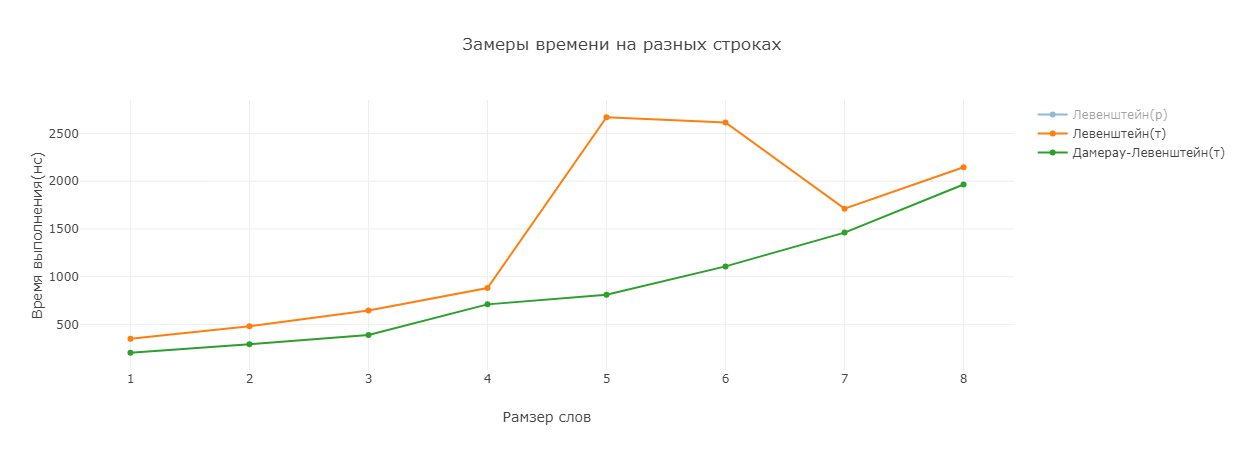
\includegraphics[width=0.8\linewidth]{images/plots_1.png}
    \vspace{5mm}
    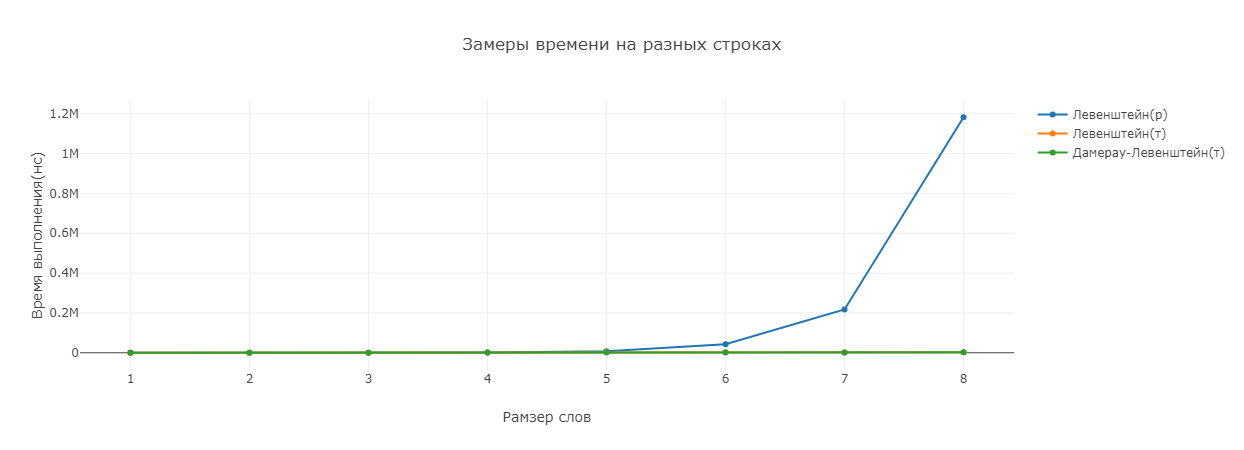
\includegraphics[width=0.8\linewidth]{images/plots_2.png}
    \caption{Сравнение алгоритмов по времени}
    \label{fig:time_measurements}
\end{figure}


\clearpage

Наиболее эффективными являются алгоритмы, использующие динамический подход (матрицу), так как в рекурсивных алгоритмах большое количество повторных расчетов.

\section{Вывод}

Рекурсивный алгоритм для вычисления расстояния Левенштейна по времени работает значительно медленнее, чем его динамический аналог. Также важно отметить, что динамические алгоритмы для расчёта расстояний Левенштейна и Дамерау-Левенштейна по времени выполнения сопоставимы между собой и примерно одинаковы.

Анализ использования памяти показывает, что рекурсивный алгоритм требует меньше памяти по сравнению с алгоритмом на основе динамического программирования. В случае динамического алгоритма для расчёта расстояния Дамерау-Левенштейна, несмотря на добавление операции перестановки символов, потребление памяти остаётся на уровне алгоритма Левенштейна, поскольку дополнительное пространство для хранения результатов перестановок не требуется.